\subsection{Consideraciones generales}
Para armar los circuitos propuestos por la cátedra se dispone de un
amplificador operacional LM-833N. Los datos más importantes a considerar
vistos en la hoja de datos son los siguientes:
\begin{enumerate}
    \item $A_{vol}$ = $110dB$
    \item BWP = $15 MHz$

\end{enumerate}    

\subsection{Circuito Derivador}
A continuación se realiza el análisis sobre el circuito derivador planteado
por la cátedra utilzando un amplificador operancional $LM833$ propuestado por 
la cátedra en el siguiente circuito.
\begin{figure}[H]
    \centering
    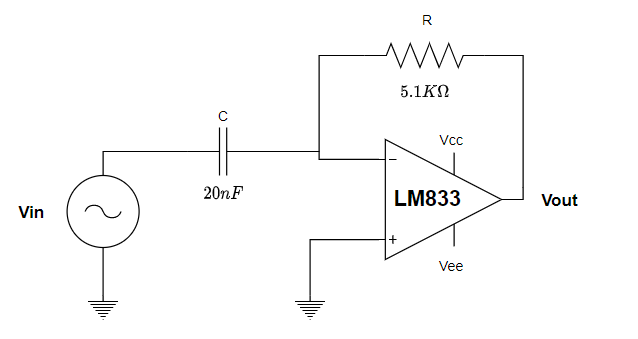
\includegraphics[width=0.6\textwidth]{../Ejercicio3-CircuitoIntegradoresyDerivadores/Imagenes/circuito_derivador.png}
    \caption{Circuito derivador implementado con Opamp}
\end{figure}

Consiguientemente, se procede a calcular la transferencia de tensión entra
la entrada y salida del circuito. \par 
En condición ideales se puede se considera que la ganancia del
amplificador operacional es infinita por lo que, basándonos en 
su ecuación característica (\ref{eq_opamp}), se puede asegurar que para 
mantener la relación $V^+=V^-$ van a tender a 0.
\vspace{2mm}
\begin{equation*}
    V_{out}=A_0(V^+-V^-)
    \label{eq_opamp}
\end{equation*}
\vspace{2mm}
Por lo tanto, se pueden escribir a las corrientes del circuito como:
\vspace{2mm}
\begin{equation*}
    I_1=\frac{V{in}}{X_c}=V_{in}\$C_1 \indent \indent I_2=\frac{V_{out}}{R}
    \label{eq_avol_ideal}
\end{equation*}
\vspace{2mm}
Considerando que $V^-=0$ y que $I_1=I_2$ se logra llegar a la transferencia bajo 
condiciones ideales:
\vspace{2mm}
\begin{equation}
    H(\$)=\frac{V_{out}}{V_{in}}=-R\$C
    \label{trans_ideal}
\end{equation}
\vspace{2mm}
Por otro lado, considerando a $A_{vol}$ finito se vuelve indispensable reformular las
ecuaciones vistas en \ref{eq_avol_ideal} ya que al considerar un $A_vol$ que no 
tiende a infinito se vuelve imposible asegurar que la tensión $V^-$ sea nula. Bajo 
las nuevas circunstancias se obtienen:
\vspace{2mm}
\begin{equation*}
    I_1=\frac{V{in}-V^-}{X_c}=(V_{in}-V^-)\$C_1 \indent \indent I_2=\frac{V_{out}-V^-}{R}
    \label{eq_avol_noideal}
\end{equation*}
\vspace{2mm}
Utilizando \ref{eq_opamp} y \ref{eq_avol_noideal} se puede despejar la transferencia
como:
\vspace{2mm}
\begin{equation}
    H_1(\$)=\frac{V_{out}}{V_{in}}=\frac{-R\$C}{1+(\frac{R\$C+1}{A_0})}
    \label{trans_no_ideal}
\end{equation}
\vspace{2mm}
Se puede validar este ecuación considerando:
 $$\lim_{A_0\to\infty} H_1(\$)$$
Se obtiene la transferencia en condiciones ideales vista en \ref{trans_ideal}. \par
Para finalizar se realiza un análisis considerando $A_{vol}$ variante en frecuencia
debido a la presencia de un polo dominante que le da una respuesta en frecuencia 
característica de un filtro pasa-bajos. La dependencia en frecuencia de la ganancia
del opamp está dada por la siguiente fórmula:
\vspace{2mm}
\begin{equation}
    A_v(\$)=\frac{A_0}{1+\frac{\$}{w_b}}
    \label{a_vol_frec}
\end{equation}
\vspace{2mm}
Siendo $A_0$ la ganancia en continua y $w_b$ el ancho de banda del filtro,
 la frecuencia para la cual el dispositivo atenúa 3 dB. \par 
 Reemplazando (\ref{a_vol_frec}) en (\ref{trans_no_ideal}) se obtiene:
 \vspace{2mm}
 \begin{equation}
    H_2(\$)=\frac{-R\$C}{1+\frac{1}{A_0}+\frac{R\$C}{A_0}+\frac{R\$^2C}{w_bA_0}}
    \label{trans_frec}
\end{equation}
\vspace{2mm}
Esta ecuación se puede dividir según su ganancia ideal $G_I$ y su factor de corrección
$F_c$ de la siguiente forma:
\vspace{2mm}
\begin{equation*}
   G_I=-R\$C \indent \indent F_c=\frac{1}{1+\frac{1}{A_0}+\frac{R\$C}{A_0}+\frac{R\$^2C}{w_bA_0}}
   \label{trans_frec}
\end{equation*}
\vspace{2mm}
Siguiendo el mismo procedimiento aplicado para $H_1(\$)$, se puede 
 $$\lim_{A_0\to\infty} H_2(\$)=\lim_{A_0\to\infty} G_IF_C=G_I=H(\$)$$

Las expresiones obtenidas se plasman en el siguiente gráfico, pudiéndose 
observar una mayor precisión a medida que se usan modelos más realistas
sin consideraciones ideales.
\begin{figure}[H]
    \centering
    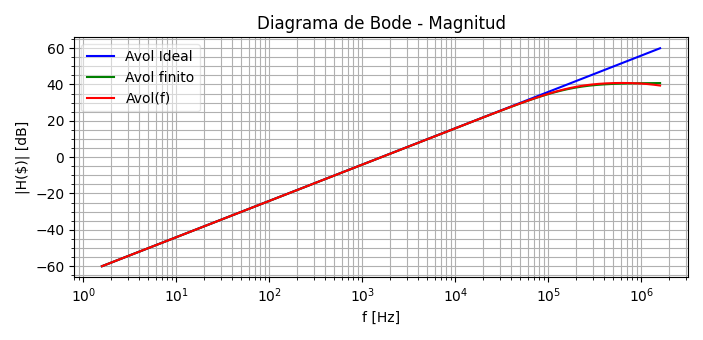
\includegraphics[width=0.6\textwidth]{../Ejercicio3-CircuitoIntegradoresyDerivadores/Imagenes/Derivador/bode_derivador magnitud.png}
    \caption{Respuesta en frecuencia teóricas - Modulo}
\end{figure}
\begin{figure}[H]
    \centering
    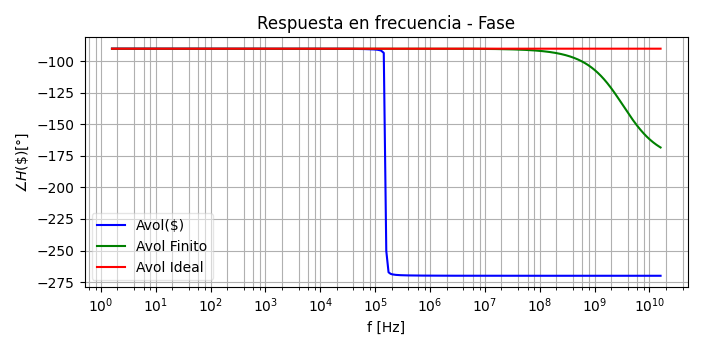
\includegraphics[width=0.6\textwidth]{../Ejercicio3-CircuitoIntegradoresyDerivadores/Imagenes/Derivador/bode_derivador_fase.png}
    \caption{Respuesta en frecuencia teóricas - Fase}
\end{figure}












\subsection{Circuito Integrador}

\subsubsection{Introducción}

Se realizó el análisis de un circuito integrador ideal, utilizando en este caso tres componentes, una Resistencia $R$,
un capacitor $C$ y un amplificador operacional. 
Cabe destacar que se considera un integrador ideal ya que a diferencia del circuito RC analizado en el primer trabajo práctico de laboratorio,
éste funcionará como integrador para cualquier frecuencia y no solo a frecuencias altas. 

Los valores nominales utilizados para la experiencia fueron:

\begin{itemize}
	\item $R: 5.1K \Omega$ 
	\item $C: 20nF$
	\item $OPAMP: LM833$
\end{itemize}

\begin{figure}[H]
    \centering 
    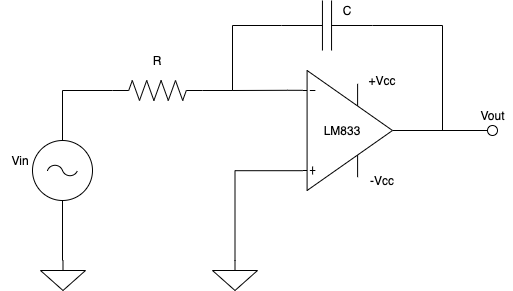
\includegraphics [scale=0.5] {../Ejercicio3-CircuitoIntegradoresyDerivadores/Imagenes/diagrama-integrador.png} 
    \caption{Diagrama del circuito integrador ideal empleado}
    \label{fig:emptyPlotTool}
\end{figure}

A continuación se procederá a calcular teóricamente el valor de las funciones transferencias para los casos en 
donde el amplificador operacional tiene un comportamiento ideal, con $A_{vol}$ finito y $A_{vol}(w)$ con polo dominante.

\subsubsection{Análisis de la Transferencia del Circuito Integrador - OPAMP ideal}

Para obtener la función transferencia en este caso, $H(S) = \frac{V_{out} (S)}{V_{in} (S)}$, partiremos de las siguientes condiciones
iniciales para el amplificador operacional:

\begin{itemize}
	\item $A_{vol}: \infty$
	\item $Z_{in}: \infty$
	\item $Z_{out}: 0$
\end{itemize}

\begin{figure}[H]
    \centering 
    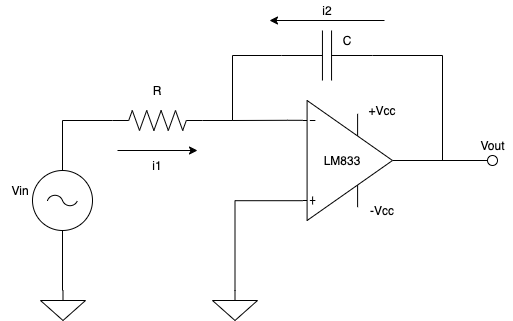
\includegraphics [scale=0.5] {../Ejercicio3-CircuitoIntegradoresyDerivadores/Imagenes/diagrama-integrador-corrientes.png} 
    \caption{Diagrama del circuito integrador ideal empleado}
    \label{fig:emptyPlotTool}
\end{figure}

Podemos observar a simple vista que:

\begin{itemize}
	\item $i1 = -i2$
	\item $i1 = \frac {V_{in}-V^{-}}{R} $
	\item $i2 = \frac {V_{out}-V^{-}}{X_c}$
	\item $V_{out} = A_{vol}(V^{+}-V^{-})$
\end{itemize}

Como ${A_{vol} \to \infty}$ y $V_{out}$ es finito, ${(V^{+}-V^{-}) \to 0}$ y como $V^{+}$ está conectado a tierra,
$(V^{-}$ representa tierra virtual, por lo cual su valor es de $0V$.

Entonces, redefiniendo las ecuaciones anteriores:

\begin{itemize}
	\item $i1 = \frac{V_{in}}{R} $
	\item $i2 = \frac {V_{out}}{X_c}$
\end{itemize}

Siendo entonces:

$$ \frac{V_{in}}{R} = - (\frac{V_{out}}{X_c}) \Longrightarrow \frac{V_{out}}{V_{in}} = -\frac{X_c}{R} = - \frac{1}{SRC}$$

$$ H(S) = - \frac{1}{SRC}$$

Claramente se puede apreciar que este circuito se comportará como un integrador, ya que si antitransformamos la función de transferencia
obtenida implicará que para obtener $v_{out}(t)$ habrá que integrar $v_{in}(t)$ en el dominio del tiempo.

En las siguientes figuras, se puede apreciar el Diagrama de Bode para este caso.

\begin{figure}[H]
    \centering 
    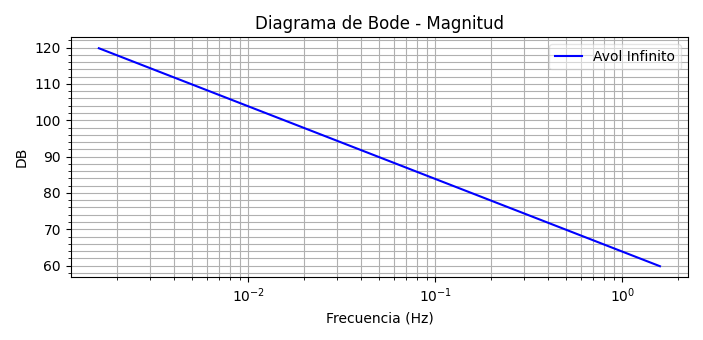
\includegraphics [scale=1] {../Ejercicio3-CircuitoIntegradoresyDerivadores/Imagenes/diagrama-bode-ideal-amplitud.png} 
    \caption{Diagrama de BODE de Amplitud para OPAMP ideal}
    \label{fig:emptyPlotTool}
\end{figure}

\begin{figure}[H]
    \centering 
    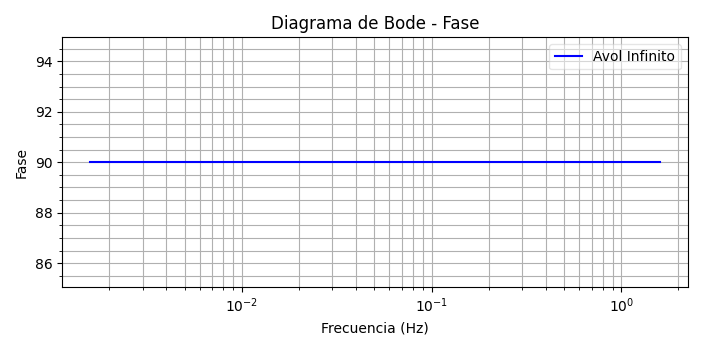
\includegraphics [scale=1] {../Ejercicio3-CircuitoIntegradoresyDerivadores/Imagenes/diagrama-bode-ideal-fase.png} 
    \caption{Diagrama de BODE de Fase para OPAMP ideal}
    \label{fig:emptyPlotTool}
\end{figure}

\subsubsection{Análisis de la Transferencia del Circuito Integrador - OPAMP con A finito}

A diferencia del caso anterior, aquí la diferencia en el cálculo de la función transferencia, $H(S) = \frac{V_{out} (S)}{V_{in} (S)}$,
entre el amplificador operaciones ideal y éste será:

\begin{itemize}
	\item $A_{vol}: finito$
\end{itemize}

Utilizando las mismas relaciones mencionadas en el apartado anterior, podemos observar ahora que:


$$V_{out}=-A_{vol}.V^{-} \Longrightarrow V^{-} = \frac{-V_{out}}{A_{vol}}$$ 


Por lo tanto:

\begin{itemize}
	\item $i1 = \frac {V_{in}-V^{-}}{R} =  \frac {V_{in} + \frac{V_{out}}{A_{vol}}}{R}$
	\item $i2 = \frac {V_{out}-V^{-}}{X_c} = \frac {V_{out} + \frac{V_{out}}{A_{vol}}}{X_c}$
\end{itemize}

Siendo entonces:

$$ \frac {V_{in} + \frac{V_{out}}{A_{vol}}}{R} = -(\frac {V_{out} + \frac{V_{out}}{A_{vol}}}{X_c})
\Longrightarrow \frac{V_{out}}{V_{in}} = \frac{1}{SCR(1+\frac{1}{A_{vol}}+\frac{1}{A_{vol}SRC})}$$

Finalmente:

$$H(S)= \frac{1}{SCR(1+\frac{1}{A_{vol}})+\frac{1}{A_{vol}}}$$

Es importante notar que siendo la ganancia para el caso ideal (GI) $- \frac{1}{SRC}$,  la funcion
transferencia se puede representar como $H(S) = GI. \frac{1}{SCR(1+\frac{1}{A_{vol}})+\frac{1}{A_{vol}}}$
Si $A_{vol}$ es lo suficientemente grande, tendremos una función transferencia ideal nuevamente.

\begin{figure}[H]
    \centering 
    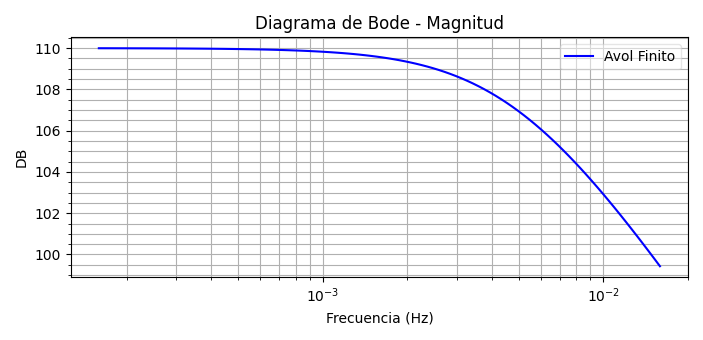
\includegraphics [scale=1] {../Ejercicio3-CircuitoIntegradoresyDerivadores/Imagenes/diagrama-bode-cideal-amplitud.png} 
    \caption{Diagrama de BODE de Amplitud para OPAMP con $A_{vol}$ finito}
    \label{fig:emptyPlotTool}
\end{figure}

\begin{figure}[H]
    \centering 
    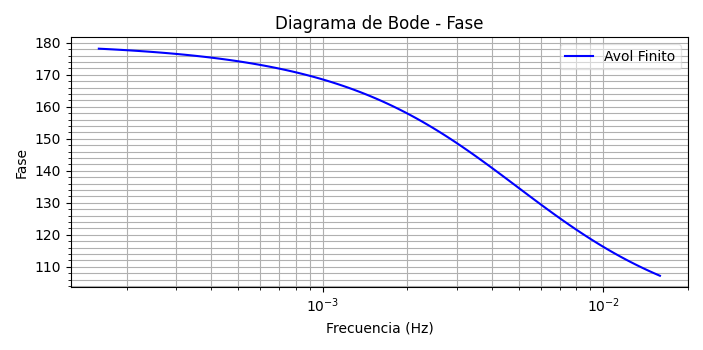
\includegraphics [scale=1] {../Ejercicio3-CircuitoIntegradoresyDerivadores/Imagenes/diagrama-bode-cideal-fase.png} 
    \caption{Diagrama de BODE de Fase para OPAMP con $A_{vol}$ finito}
    \label{fig:emptyPlotTool}
\end{figure}

\subsubsection{Análisis de la Transferencia del Circuito Integrador - OPAMP con $A_{vol}(w)$}

En este ultimo caso de analisis, $A_{vol}$ no es constante sino que es función de la frecuencia según:

$$A_{vol}=\frac{A_0}{1+\frac{S}{w_b}}$$

Por lo cual la expresion para la funcion transferencia calculada en el caso anterior, quedara denominada por:

$$H(S)= \frac{1}{SCR(1+\frac{1+\frac{1}{SCR}}{A_{vol}})}\Longrightarrow H(S)= \frac{1}{SCR(1+\frac{1+\frac{1}{SCR}}{\frac{A_0}{1+\frac{S}{w_b}}})}$$ 

Reacomodando algebraicamente:

$$H(S)=- \frac{1}{S^2\frac{CR}{A_oW_b}+SCR(1 + \frac{1}{A_o}+\frac{1}{W_bA_oCR}) + \frac{1}{A_0}}$$

Podemos observar que si $A_o$ es muy grande, nuevamente estaremos en el caso donde la ganancia que obtendremos será la ideal para este circuito.

\begin{figure}[H]
    \centering 
    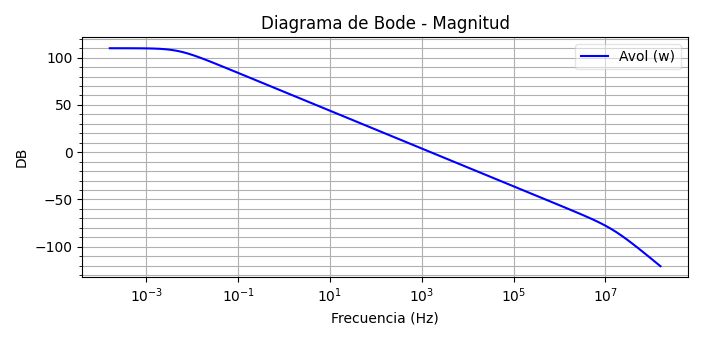
\includegraphics [scale=1] {../Ejercicio3-CircuitoIntegradoresyDerivadores/Imagenes/diagrama-bode-noideal-amplitud.png} 
    \caption{Diagrama de BODE de Amplitud para OPAMP con $A_{vol}(w)$ finito}
    \label{fig:emptyPlotTool}
\end{figure}

\begin{figure}[H]
    \centering 
    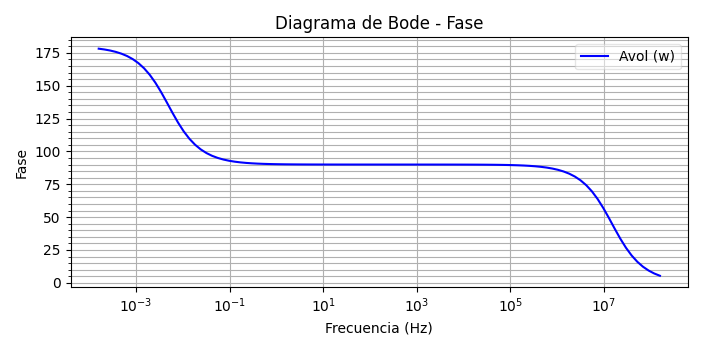
\includegraphics [scale=1] {../Ejercicio3-CircuitoIntegradoresyDerivadores/Imagenes/diagrama-bode-noideal-fase.png} 
    \caption{Diagrama de BODE de Fase para OPAMP con $A_{vol}(w)$ }
    \label{fig:emptyPlotTool}
\end{figure}

Comparando los tres casos, podemos observar que en determinadas frecuencias el comportamiento es identico:

\begin{figure}[H]
    \centering 
    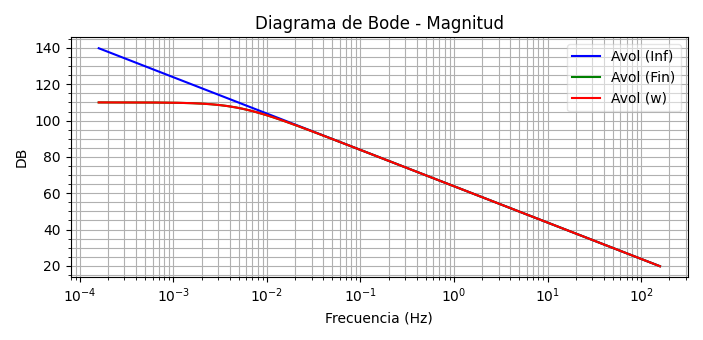
\includegraphics [scale=1] {../Ejercicio3-CircuitoIntegradoresyDerivadores/Imagenes/comparativo-magnitud.png} 
    \caption{Diagrama de BODE de Amplitud para OPAMP comparativo }
    \label{fig:emptyPlotTool}
\end{figure}

\begin{figure}[H]
    \centering 
    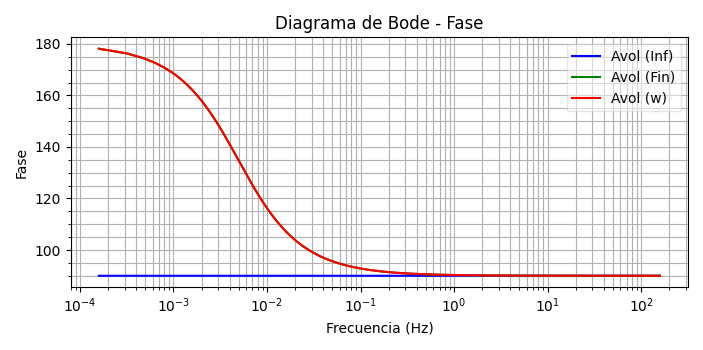
\includegraphics [scale=1] {../Ejercicio3-CircuitoIntegradoresyDerivadores/Imagenes/comparativo-fase.png} 
    \caption{Diagrama de BODE de Fase para OPAMP comparativo }
    \label{fig:emptyPlotTool}
\end{figure}

\subsubsection{Análisis de Impedancia de Entrada al Circuito Integrador}

Para poder calcular teoricamente, la impedancia de entrada, $Z_{in}$, se utilizó el teorema de Miller tal que:

